\hspace*{0.7in} Graphical user interface is designed and which is expressed through some screen shots using HTML and Java. The experiments carried out with the system are shown below with the help of graphical user interface of the system.
\begin{figure}[h]
\centering
  % Requires \usepackage{graphicx}
  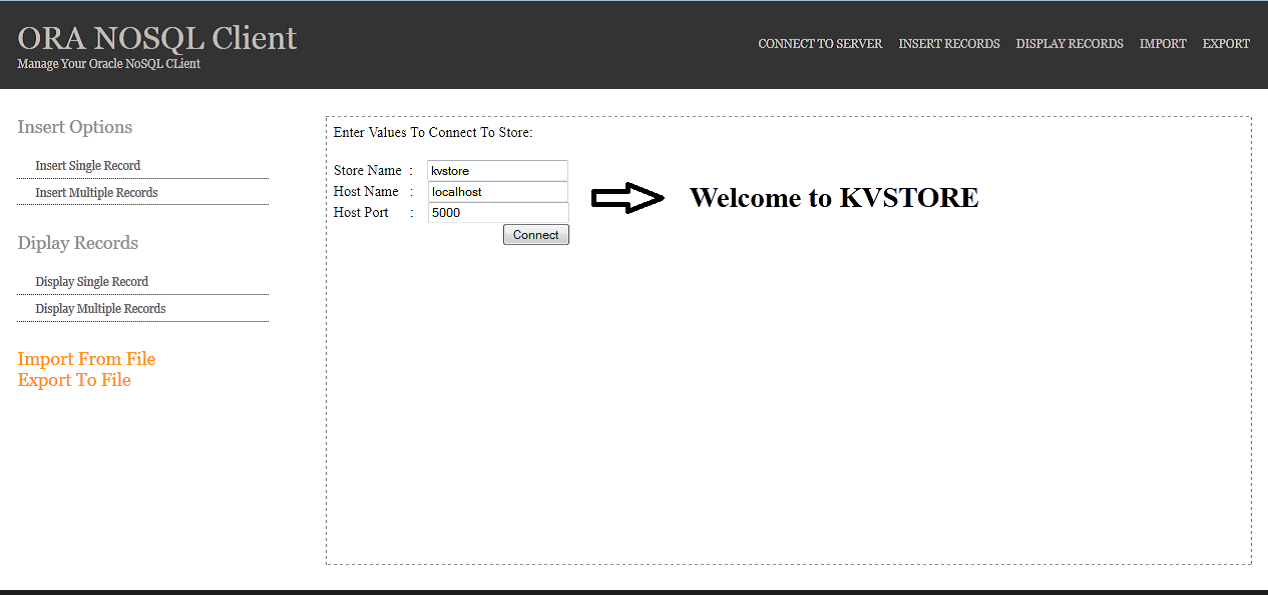
\includegraphics[width=13cm,height=7cm]{ERD1.png}
  \caption{Working Model of System.}\label{Working Model of System.}
\end{figure} \\
As the system was tested locally, it is capable of performing every operation listed above. The system is deployed on Glassfish Server and the results were good to compare with. Simultaneously various clients were connected and operations were performed and the System worked fine with that.\\

\newpage
\begin{figure}[h]
\centering
  % Requires \usepackage{graphicx}
  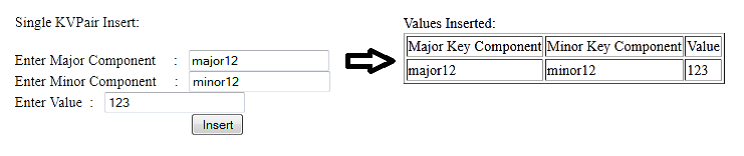
\includegraphics[width=13cm,height=3.5cm]{ERD2.png}
  \caption{Single KVPair Insert Operation}\label{Single KVPair Insert Operation}
\end{figure}
Above Figure shows Single KVPair insert and the same is applied for Multiple KVPair insert, but only first time the Major Key component and Number of Minor Key Components is asked and that number of fields is generated for user to insert value.

\begin{figure}[h]
\centering
  % Requires \usepackage{graphicx}
  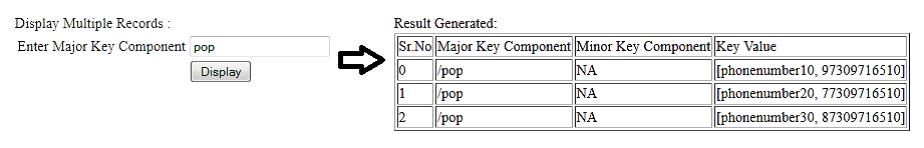
\includegraphics[width=13cm,height=3.5cm]{ERD3.png}
  \caption{Multiple KVPair Display Operation}\label{Multiple KVPair Display Operation.}
\end{figure}
Above Figure shows Multiple KVPair Display operation, same applies for Single KVPair display, but there user has to specify Major as well as Minor Key Component.

\begin{figure}[h]
\centering
  % Requires \usepackage{graphicx}
  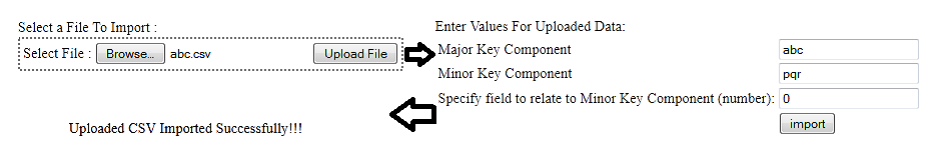
\includegraphics[width=13cm,height=3.5cm]{ERD4.png}
  \caption{Import CSV Operation.}\label{Import CSV Operation.}
\end{figure}
Above Figure shows Import Data from CSV operation, here the CSV file is uploaded to server and then user has to specify Major and Minor Key Component along with the index of field which is to be associated with Minor Key Component. \\
For Export Data to file, the user first has to perform Single or Multiple Display Operation and after that a link is provided, through which the user can download generated CSV file. \\ \\
Below are the Screen shots of Android Application, which is developed to consume the web services. This application is used for getting attendance report of the user.
\begin{figure}[h]
\centering
  % Requires \usepackage{graphicx}
  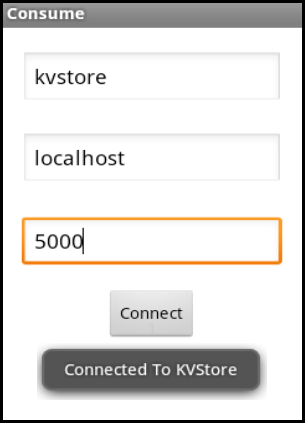
\includegraphics[width=6cm,height=7cm]{ERD5.png}
  \caption{Interface for connection to Store.}\label{Interface for connection to Store.}
\end{figure}
\\
\\
\\
\\
\begin{figure}[h]
\centering
  % Requires \usepackage{graphicx}
  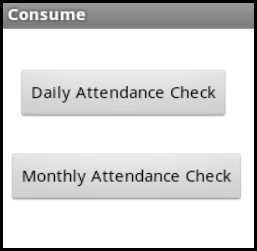
\includegraphics[width=6cm,height=7cm]{ERD6.png}
  \caption{Options for Attendance Check.}\label{Options for Attendance Check.}
\end{figure}

\newpage
\begin{figure}[h]
\centering
  % Requires \usepackage{graphicx}
  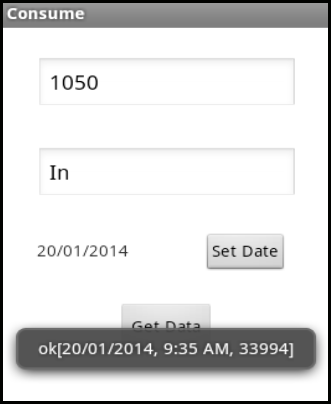
\includegraphics[width=6cm,height=7cm]{ERD7.png}
  \caption{Daily Attendance Check Interface.}\label{Daily Attendance Check Interface.}
\end{figure}

\begin{figure}[h]
\centering
  % Requires \usepackage{graphicx}
  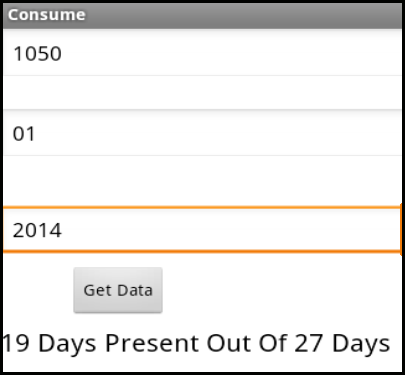
\includegraphics[width=6cm,height=7cm]{ERD8.png}
  \caption{Monthly Attendance Check Report.}\label{Monthly Attendance Check Report.}
\end{figure}
\hspace*{0.7in} In this way the experiments are carried out on every functions of the system and we have found various results as shown in above screenshots. The system works well. 